% Objective of the paragraph: setup the hype context and importance of the problem
Reinforcement learning (RL) is an exciting field of research as it allows for
agents to learn complex behaviors in a multitude of environments while requiring
minimal supervision in the form of reward signals. This is readily
evidenced from RL's recent successes in various domains ranging from goal-agnostic ones such as  
playing Atari games~\cite{MnKaSiNATURE2015} from purely visual input and defeating world GO
champions~\cite{gibney2016google}, to goal-driven ones such as recent
applications in robotic navigation~\cite{mirowski2018learning} and
manipulation~\cite{pong2018temporal}. In the realm of multi-goal tasks, this
work introduces Floyd-Warshall Reinforcement Learning (FWRL), a new algorithm
that allows transferring learned behaviours in environments with dynamic goal
locations.


% brief background on model-based and model-free learning.
Algorithms in RL are often classified as being either
\emph{model-based} or \emph{model-free}, the distinction being whether
an environment state-transition function is learned explicitly or
implicitly.  In \emph{model-based} RL, the dynamics that govern an
environment's transitions is explicitly modelled.
At any point in an episode, agents use this model to
predict future states and utilize this information to maximize possible
reward. This formulation is known to be sample-efficient while normally
not achieving high asymptomatic performance~\cite{pong2018temporal}.
In contrast, in \emph{model-free} RL, algorithms such as policy gradients,
actor-critic and Q-learning directly learn the expected ``value'' for each
state without explicitly learning the environment-dynamics. This paradigm has
been behind most of the recent success stories of high performance in diverse
applications like Atari games, Go championships etc.

\begin{figure}%
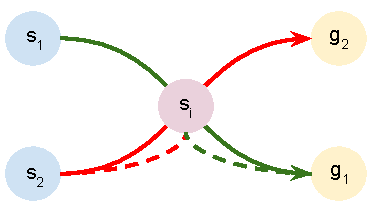
\includegraphics[width=\columnwidth]{./media/optimal_trajectories.pdf}\\
\caption{The intuition driving the workings of FWRL. An agent is
independently directed to goal state 1 from start state 1 and goal state
2 to start state 2. The agent is then directed to traverse to goal state
1 from start state 2. Intuitively, the agent can use the previous
trajectories to find a shorter path to perform this traversal (the
dotted line). However, standard Q-Learning discards all previous
experience during learning. FW Learning utilizes such shortest path
based constraints to find goal locations faster.  }
\label{fig:ql-fw-grid-world-results}%
\end{figure}

% Goal-conditioned tasks
Many problems in robotics, like navigation, and  pick and place tasks can be
formulated in multi-goal domains where the task to be completed requires the
specification of goal information. However, for such tasks model-free RL struggles
to transfer learned behavior from one goal location to another within the same
environment~\citep{dhiman2018critical}. This happens because model-free RL represents the environment as
value functions which conflate the state-dynamics and reward distributions into
a single representation.
On the other hand, while model-based RL allows for the separation of environment
dynamics and reward, small errors in the modelling function lead to significant
drops in performance.

We are interested in improving the performance of model-free algorithms
in multi-goal domains while retaining the high asymptotic performance
afforded in single goal tasks. Much prior work has attempted to do this. 
To address the performance of model-free RL for multi-goal RL problems, we take
inspiration from the Floyd-Warshall shortest path algorithm~\cite{floydwarshall1962}.
Floyd-Warshall is a generalization of Dijkstra's algorithm that computes the
shortest path from every node in a graph to all other nodes.
This work introduces Floyd-Warshall Reinforcement Learning, a new algorithm for
model-free RL in multi-goal tasks. FWRL works by
modeling a goal-conditioned action-value function where every state in the state
space can be a valid goal. This allows FWRL to remember the paths even if they
do not lead to the goal location during a particular episode. 

% Related Work - where are we coming from 
Similar attempts have been made to retain the high asymptotic
performance of model-free algorithms on multi-goal tasks.
\citet{schaul2015universal} introduce goal-conditioned value functions
that generalize across both state and goal spaces allowing for
making goal-specification explicit in RL domains. In temporal difference
modelling, equivalences between model-based and model-free algorithms
are proposed and utilized to bootstrap Q-learning. The algorithm is
conditioned on the horizon. In Hindsight Experience Replay, previous
failed traversals are re-imagined as succesful leading to significant
increases in learning times. While these methods have shown success in
many environments, they are concerned with using Q-functions to estimate
goal conditioned action-value functions. In contrast, our algorithm
proposes the FW function as an alternative. This motivation is
similar to the Hindsight Experience Replay \cite{anderson2017vision}, however,
we use the transitive relation between goal-conditioned value function which
allows us to utilize hindsight experience in more fine-grained manner.

Experimentally, FWRL is shown to outperform model-based and model-free
algorithms in a tabular setting. FWRL is found to outperform the next
most significant baselines by as much \TODO{x\%}.


%Recently, a few works have used the idea of goal-conditioned value functions. In
%Temporal-Difference modelling \cite{pong2018temporal} model a goal conditioned
%action-value function that is also conditioned on the horizon. In contrast our
%proposed value function is independent of horizon length, and hence easier to
%estimate.



